\documentclass[12pt]{article}
\usepackage{wkrpt}
\begin{document}

\title{An Analysis of Global Scoped CSS and Atomic CSS in the Context of Styling Component Based Applications}
{
	Yahoo!\\
	Sunnyvale, CA
}
{
	Aditya Sridhar\\
	3B Software Engineering\\
	Student ID 20539123\\
	User ID a3sridha\\
	September 30, 2016
}


\letter{An Analysis of Global -Scoped CSS and Atomic CSS in the Context of Styling Component Based Applications}{3B}{Yahoo!}{Mail Frontend}
{
	\noindent
	Aditya Sridhar\\
	201 Lester Street\\
	Waterloo, ON N2L 3W3
}
{
	\noindent
	This report, entitled \textit{“An Analysis of Global Scoped CSS and Atomic CSS in the Context of Styling Component Based Applications”}, was prepared during my 3B work term at Yahoo!, where I worked for the Yahoo! Mail frontend team.
}
{
	\noindent
	The Yahoo! Mail frontend team is currently developing the next generation web client of Yahoo! Mail built using React. I was responsible for building many user facing as well as core features on the mail web client.
}
{
	\noindent
	The frontend engineers at Yahoo invented the Atomic CSS paradigm to improve maintainability of style sheets in component based projects. This was done mainly to solve many problems with regards to maintaining global style sheets. This report compares the global scoped CSS method with the Atomic CSS method against a set of five evaluation criteria and identifies the more appropriate solution.
}
{
	\noindent
	I would like to thank my manager, Mr Mohit Goenka for assigning me the responsibility of implementing critical features that will be used by hundreds of millions of users. I would also like to thank my team for encouraging me to follow good design practices while implementing the features I was assigned.
}


\tocsection{Executive Summary}

The next major revision of Yahoo Mail is built on React. React is a JavaScript framework used to build component based web application. The idea is that a component is responsible for a single part of the user interface. Style rules are written in CSS files which target a particular element in the web page content markup that is to be styled. This report compares two different methods used to style web page content in a component based application.

Maintainability is a major issue that is associated with CSS. It significantly affects all the developers in the team as it hampers project scalability. As the size of a project grows, maintainability of style sheets become harder. Low reusability of styles is one of the factors contributes to the degradation of maintainability. This report discusses other factors that affect maintainability in detail. This report also implores how changing the scope of styles in a style sheet can lead to an improvement in maintainability of the style sheets.

A set of design constraints was noted and solutions satisfying the constraints were compared. The report compares two different solutions against a set of five evaluation criteria: minimal contextual styling, style simplicity, style reusability, low specificity and separation of content and style. The report leverages Analytical Hierarchical Process  (AHP), a technique used to perform quantitative analysis of two solution against a set of evaluation criteria. 

Finally, the report recommends the use of Atomic CSS method to style web pages in a component based application. It is also highly recommended to maintain a one-to-one mapping between styles and class names. This will increase the modularity of an application and will enable developers to maintain components instead of style sheets.

\newpage

\toc
\lof
\lot

\pagenumbering{arabic}
\section{Introduction}
\subsection{Background Information}

Yahoo! is a technology company and is recognized as one of the pioneers of the early-internet era. Yahoo! Mail is a web-based email service owned by Yahoo! with hundreds of millions of users worldwide [1]. The next generation of Yahoo! Mail web client is currently being developed and is built using the React framework. React is a component based JavaScript library used for building user interfaces. The idea behind a component based framework is that a complex user interface should composed of multiple components, and each component should follow the Single Responsibility Principle (SRP). This implies that a particular component should be responsible for a single part of the user interface.

\vspace{0.5cm}

\begin{table}[h]
	\centering
	\begin{tabular}{|c|c|}
		\hline
		\textbf{Concern} & \textbf{Resource} \\ 
		\hline
		Presentation & CSS \\
		\hline 
		Structure & HTML \\
		\hline
		Behaviour & JavaScript \\
		\hline
	\end{tabular}
	\caption{SoC principle in the context of web development}
\end{table}

\vspace{0.5cm}

Traditionally, the development of web pages was based on the principle of Separation of Concerns (SoC) which advocates breaking a problem into different concerns and using a resource to address a particular concern [2]. In the context of web pages, the structure, presentation and behaviour layers were identified as separate concerns with Hyper Text Markup Language (HTML) defining the structure of a web page, Cascading Style Sheets (CSS) defining the content presentation styles and JavaScript (JS) defining how a web page behaves with user interaction. Table 1.1 summarizes the SoC principle in the case of web page development.

\subsection{Introduction to the Issue}
CSS is a collection of rules, each rule containing one or more selectors and a block of styles. These rules are written in style sheets which are then packaged in the main project. A selector is used to identify a particular HTML element in the web page content and the styles specified in the rule are applied to that particular HTML element. Figure 1.1 better elaborates how CSS rules work. The selector \textit{div} targets the \textit{<div>} HTML element and the styles mentioned in the corresponding style block are applied to the targeted HTML element.

\vspace{0.5cm}

\begin{figure}[h]
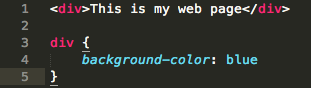
\includegraphics[scale=0.7]{selector-normal}
\centering
\caption{Example of styling using CSS selectors}
\end{figure}

\vspace{0.5cm}

The scope of a CSS rule is a portion of the web page where that rule can be used to style an element on the web page. The rules contained in a global-scoped style sheet can be used to style any element on the web page. Hence the scope of the rules in a global style sheet is not limited to a particular portion of the web page. Atomic CSS on the other hand, is a design principle that advocates restricting the scope of a CSS rule to a component of the web page [3].

This report compares CSS in global style sheets with Atomic CSS in the context of styling component based applications. It first provides some additional information about the issue and lists a set of design constraints and the evaluation criteria. It identifies the benefits and pitfalls of each accepted solution. The report uses AHP to perform quantitative analysis of the alternatives against a set of evaluation criteria. The report then concludes by identifying the best solution and provides some recommendations.

\newpage

\section{Problem Specifications}
\subsection{Problem Description}
CSS is an important component of the frontend toolkit. Since the internet is composed of billions of web pages [4], CSS is being used on a regular basis to govern the look and feel of web pages. One of the main concerns of using CSS is maintainability. CSS is easy to maintain when the web pages have less content, but as the size of the project increases, the maintainability of style sheets decreases. High maintainability implies that a developer can modify a particular rule without worrying about it adversely impacting other style rules. Low maintainability hampers the scalability of a project from a design standpoint and significantly affects the developers in the team.

As mentioned earlier, a CSS selector targets a particular HTML element in the web page content and the styles linked to the selector are applied to the element it targets. As the content of the web page grows, CSS selectors are more specific and descriptive to target a particular element in the web page. This is termed as selector specificity. If two selectors target the same element in the web page content, the selector with higher specificity tends to override the selector with lower specificity. The style sheet containing selectors with high specificity makes it harder for an existing style to be overriden by a new style. Hence low specificity leads to high maintainability.

\begin{figure}[h]
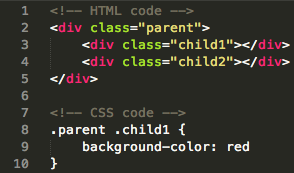
\includegraphics[scale=0.7]{descendent-selector}
\centering
\caption{Example of styling using context-based selectors}
\end{figure}

At times, a developer might want to match a web page element that is a descendent of another web page element. For example in Figure 2.1 the \textit{<div>} element whose class name is \textit{child1} is a descendent of the \textit{<div>} element whose class name is \textit{parent}. The CSS selector \textit{.parent .child1} is an example of a context-based selector. It is targeting the element with class name as \textit{child1} that is a descendent of the element with class name as \textit{parent}. This means that the descendent element is being styled in the context of its parent, and that the rule is redundant outside of this context. This will ultimately lead to more rules being added to the style sheet if the requirement to style the same element outside of the context arises.


% TODO: add one more para

% As the number of rules in a style sheet increases, the maintainability decreases. Hence making the styles reusable makes the stylesheets more maintainable. ... Intutive thing ... 


% what is context based styling and descendent selectors and how does it affect maintainablility



% how decoupling .... makes.... 
% why is maintainablity affected
% why context based styling affects maintainabliity..


% In problem description mainly talk about maintainability, and talk about how disadvantages of global CSS leads to maintainability issues. Also introduce topics like contextual selectors



% TODO: explain different types of selectors, explain contextual styling

% IMPORTANT POINT: reducing the scope improves maintainability significantly

\subsection{Design Constraints}
A solution should adhere to the following design constraints, in order to be deemed as an accepted solution:
\begin{enumerate}

	\item The styles should be able to be overriden by other styles if required. That is, the selector must not have the highest specificity.

	\item The styles should be able to be applied using class selectors.

\end{enumerate}
% Design constraints: 1) If change occurs, should not be applied to every element 3) Ability to style using classes. Refer to https://vineetgupta22.wordpress.com/2011/07/09/inline-vs-internal-vs-external-css/


\subsection{Design Criteria}
Reusability and maintainability are important features in the context of component based applications. The following evaluation criteria were designed keeping these features in mind and are used to compare and analyze the two accepted solutions.
\begin{enumerate}

	\item \textbf{Minimize the usage of context-based styling}: The accepted solution should limit the usage of contextual styling as this demotes reusability and portability of styles. This ultimately makes style sheets hard to maintain.
	% Note: this can be done by limiting the use of descendent selectors. say in global approach this could be kept in mind but hard to enforce as projects grow. In atomic approach this never happens

	\item \textbf{Low specificity of styles}: Low CSS specificity enables the developer to override a CSS rule when requirements change. This makes the style sheets more maintainable.

	\item \textbf{Intuitive style changes}: The accepted solution should be intuitive and predictable enough for the developer to visualize any changes made to the style sheet in terms of web page presentation. This includes adding, removing and modifying rules.

	\item \textbf{Style reusability}: The accepted solution should promote reusability of styles. New style requirements being added to the specification should sparingly lead to new rules being added to the style sheet.

	\item \textbf{Decouple markup and styles}: The accepted solution should disallow coupling of web page content (markup) and styles. This enables the developer to make changes to the presentation without making changes to the markup.

\end{enumerate}

\subsection{Evaluation Process}
This report leverages AHP, a Multi-Criteria Design Analysis (MCDA) approach used to convert a set of qualitative comparisons into quantitative scores. The first step of AHP involves establishing a rating scale as illustrated in Table 2.1.

\begin{table}[h]
	\centering
	\begin{tabular}{|c|c|}
		\hline
		\textbf{Rating} & \textbf{Interpretation} \\ 
		\hline
		1 & Equally preferable \\
		\hline 
		2 & Slightly preferable \\
		\hline
		3 & Significantly preferable \\
		\hline
	\end{tabular}
	\caption{Rating scale}
\end{table}

Next, the rating scale is used to analyze each evaluation criteria and quantify the relative importance of each criterion. This is illustrated in Table 2.2

\begin{table}[h]
	\centering
	\begin{tabular}{|c|c|}
		\hline
		\textbf{Criterion} & \textbf{Relative Importance} \\ 
		\hline
		Minimal contextual styling & 10.7\% \\
		\hline 
		Low specificity & 10.7\% \\
		\hline
		Style simplicity & 7.5\% \\
		\hline
		Style reusability & 41.2\% \\
		\hline
		Separation of content and style & 29.9\% \\
		\hline
	\end{tabular}
	\caption{Criteria weighting}
\end{table}

Finally, the score for each alternative is calculated for each criterion. The summation of scores for each criterion is the final score of the alternative. The final scores are compared to identify the more appropriate solution.

\newpage

\section{Accepted Solutions}
\subsection{Global Scoped Style Sheets}
\subsubsection{Explaination}
Before CSS was invented, styles were written directly on the HTML markup, resulting in web page content and styles being tightly coupled with each other. As the use of the internet evolved, styles were isolated in style sheets by virtue of the SoC principle. These style sheets had a global scope and the rules present in these style sheet can be used to style any element in the web page content. Since the scope is not limited to a particular portion of the web page, the usage of context-based selectors is inevitable as the size of the project grows. As an example consider the case in Figure 3.1. The CSS selector is targetting the \textit{<p>} element and setting its font size to be 10 pixels.

\vspace{0.5cm}

\begin{figure}[h]
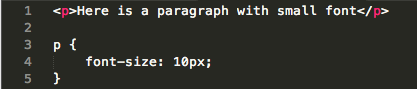
\includegraphics[scale=0.7]{global-scope-one}
\centering
\caption{Plain selector targetting \textit{<p>} element}
\end{figure}

\vspace{0.5cm}

\begin{figure}[h]
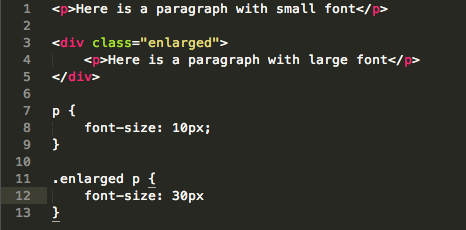
\includegraphics[scale=0.7]{global-scope-two}
\centering
\caption{Context-based selector targetting \textit{<p>} element}
\end{figure}

\vspace{0.5cm}

A new requirements demands all \textit{<p>} elements contained inside a \textit{<div>} element with class name as \textit{enlarged} to have a font size of 30 pixels. To override the existing style targetting all \textit{<p>} elements, the usage of  context-based selector as illustrated in Figure 3.2 cannot be avoided. It can noted that the specificity of the new selector has also increased, making it harder to be overriden in the future. 

%Finally, since the scope is not limited, reusability is a concern .. 

\subsubsection{Advantages}
The following are the advantages of using global-scoped style sheets:
\begin{enumerate}
	\item Web page styles are decoupled from the markup allowing for a more flexible development with less refactoring. Changes made to the markup do not often lead to changing of styles and vice-versa.

	\item This approach introduced the usage of selectors to target a particular element in the web page markup. This enabled matching markup elements with similar styles and styling them all at once, improving reusability considerably.
\end{enumerate} 

\subsubsection{Disadvantages}
The following are the disadvantages of using global-scoped style sheets:
\begin{enumerate}
	\item Since scope of CSS rules is not restricted to a particular section of the web page, the usage of context based selectors is unavoidable as size of the project grows.

	\item CSS selectors tend to be more descriptive as size of the project grows. Hence CSS selector specificity is high.

	\item CSS rules are not intuitive as the effect made by a context-based CSS rule on the presentation of a web page element is hard to visualize.
\end{enumerate}

\subsection{Atomic CSS}
\subsubsection{Explanation}
Atomic CSS advocates restricting the scope of a CSS rule to a component of the application [3]. It was invented by engineers at Yahoo! primarily to adopt a more modular approach to maintaining style sheets. This approach was found to thrive in the context of component based technologies like React. This approach violates the SoC principle since a component's presentation is mixed with its structure. However this is logically appropriate in the context of component based applications as a component is considered an independent view that handles its own behaviour and application state. Hence this approach enables a developer to maintain components instead of maintaining style sheets.

\vspace{0.5cm}

\begin{figure}[h]
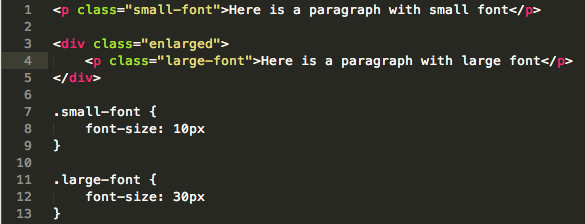
\includegraphics[scale=0.7]{atomic-css}
\centering
\caption{Atomic CSS method}
\end{figure}

\vspace{0.5cm}

This method promotes the use of unsemantic class names [3]. There is a one-to-one relationship between a style and a class name. Hence the styles are context agnostic improving their reusability dramatically. Figure 3.3 is an example of how one can style web pages using the Atomic CSS method. The specifications of this example is the same as that in Figure 3.2. Here, a class name is allocated for each style and the styles are not contextual. The specificity of the styles is also low. Further, since the styles are devoid of a context, they can be reused in other parts of the component.

\subsubsection{Advantages}
The following are the advantages of using the Atomic CSS method:
\begin{enumerate}
	\item Since CSS styles are context agnostic, they can be used to style a particular HTML element in the component without the usage of context-based selectors.

	\item Owing to the one-to-one relationship between styles and class names, a CSS selector need not be descriptive when targetting a particular HTML element in the component. Hence specificity of a selector is low, allowing for easier style overrides in the future.

	\item The effect made by a CSS rule on a component's presentation is easy to visualize. This makes it easier to identify and clean up rules that are obsolete.
\end{enumerate}


\subsubsection{Disadvantages}
The following are the advantages of using the Atomic CSS method:
\begin{enumerate}
	\item This method does not follow the SoC principle to some extent as a component's presentation is linked with its behaviour and structure. Hence a change made to a style often leads to changes being made to the component's markup

	\item HTML5 documentation promotes the use of semantic class names and states that a class name should be reflective of the element's behaviour instead of describing an element's presentation [7]. This is being violated by the Atomic CSS approach as class names are used to describe an element's style.
\end{enumerate}

\newpage

\section{Alternative Not Considered}
\subsection{Explanation}
This method is used to apply styles directly to an HTML element [8] and is named the Inline CSS method. Hence styles and markup are tightly coupled together. Figure 4.1 illustrates how to style a particular HTML element using the Inline CSS method. The style attribute is used to record an element's styles. Inline CSS have the highest specificity and will have precedence over other methods used to style web page content. This was one of the earliest methods to style web pages and was soon replace by external style sheets. Today, it is considered a bad practice to use this method to style web pages.

\vspace{0.5cm}

\begin{figure}[h]
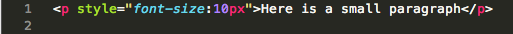
\includegraphics[scale=0.7]{inline-css}
\centering
\caption{Inline CSS method}
\end{figure}

\subsection{Advantages}
There are limited advantages to the Inline CSS method.
\begin{enumerate}
	\item Since they have the highest precedence, they can be used to try out a particular style on an element to determine if its the right fit or not.
\end{enumerate}

\subsection{Disadvantages}
The following are the disadvantages of the inline CSS method
\begin{enumerate}
	\item Inline styles have the highest specificity, making them hard to be overriden by other styles.

	\item This method leads to poor reusability of styles. Styles must be specified using the style attribute for every occurence of the target element in the markup.
\end{enumerate}


\newpage

\section{Results}
Since the two solutions are compared against a set of relatively subjective evaluation criteria, AHP is the most suitable MCDA method of quantitative analysis. The alternative score for each criterion is calculated and is then multiplied with the criterion’s weighting to obtain a final score of each alternative for each criterion. \textbf{Table 5.1} represents a set of final scores. Figure 5.1 is the graphical representation of the set of final scores.

\vspace{0.5cm}

\begin{table}[h]
	\centering
	\begin{tabular}{|c|c|c|}
		\hline
		\textbf{Criterion} & \textbf{Atomic CSS} & \textbf{Global CSS} \\ 
		\hline
		Minimal contextual styling & 0.086 & 0.021 \\
		\hline 
		Low specificity & 0.086 & 0.021 \\
		\hline
		Style simplicity & 0.050 & 0.025 \\
		\hline
		Style reusability & 0.276 & 0.136 \\
		\hline
		Separation of content and style & 0.060 & 0.239 \\
		\hline
		\textbf{Total (in \%)} & \textbf{55.8} & \textbf{44.2} \\
		\hline
	\end{tabular}
	\caption{Final scores}
\end{table}

\vspace{0.5cm}

\begin{figure}[h]
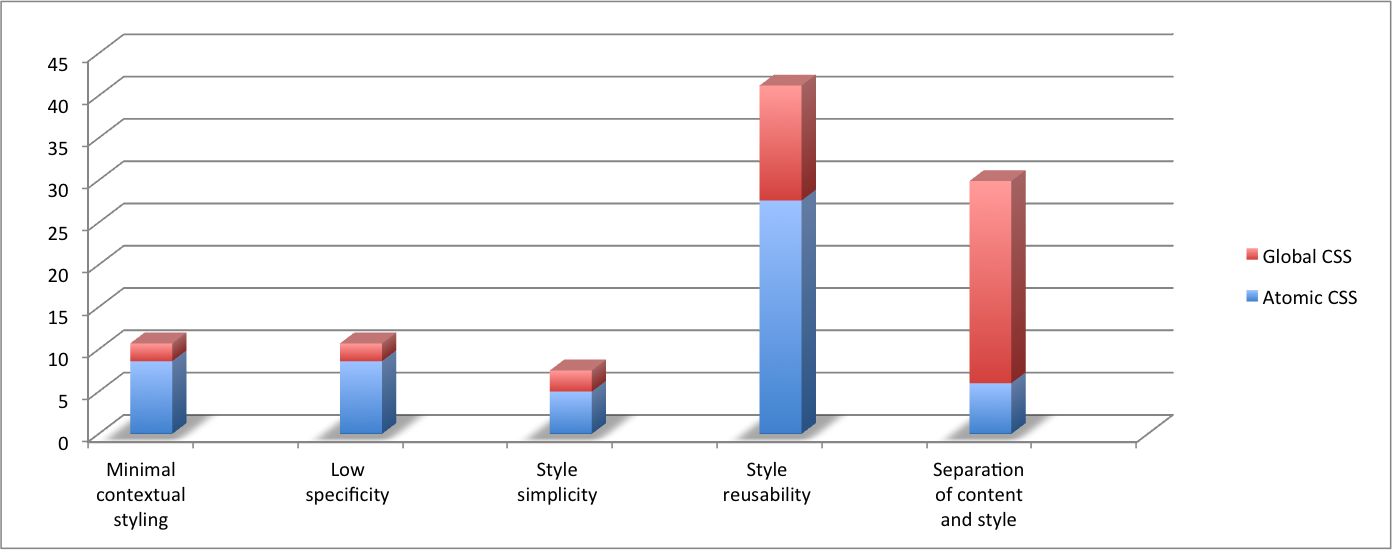
\includegraphics[scale=0.7]{chart}
\centering
\caption{Graphical representation of final scores}
\end{figure}

\vspace{0.5cm}

\newpage

\section{Conclusions}
All the solutions were judged primarily on context-based styling usage, selector specificity, style simplicity, style reusability and content-style separation. The accepted solutions, the Global CSS method and the Atomic CSS method, were found to satisfy all the design constraints whereas, the rejected solution, the Inline CSS method, was found not to satisfy the design constraints. The report utilizes AHP to perform a robust, quantitative analysis of the two techniques while dealing with multiple evaluation criteria.

The results indicate that the Atomic CSS method fared significantly better than the Global CSS method when compared on the basis of context-based styling usage, selector specificity and style simplicity. On the basis of style reusability, the Atomic CSS method performed marginally better than the Global CSS method. However, on the basis of content and style separation, the Global CSS method was found to perform significantly better than the Atomic CSS method. Ultimately, this report concludes that the Atomic CSS method should be preferred over the Global CSS method.

\newpage

\section{Recommendations}
This report recommends using the Atomic CSS method to style content in component based applications. Having a one-to-one mapping between styles and class names is highly recommended. Removing obsolete styles from style sheets is also recommended as it increases maintainability. Developers are encouraged to follow the ideology of maintaining components and not style sheets, as Atomic CSS is found to work best with this modular approach.

It is also recommended to maintain a global style sheet containing a list of constant styles, as this helps maintain uniformity across components. For example if the colour of the text displaying error message is red across all components, it could be accessed from a global style sheet by a component when needed. 

\newpage

\section{References}

\begin{enumerate}

	\item \myurl{en.wikipedia.org/wiki/Yahoo!_Mail}

	\item \myurl{en.wikipedia.org/wiki/Separation_of_concerns}

	\item \myurl{acss.io/frequently-asked-questions.html#what-is-atomic-css-}

	\item \myurl{internetlivestats.com/total-number-of-websites/}

	\item \myurl{smashingmagazine.com/2013/10/challenging-css-best-practices-atomic-approach/}

	\item \myurl{fullstackforum.com/software/2015/07/14/styling-in-react-and-atomic-css/}

	\item \myurl{www.w3.org/TR/html5/dom.html#classes}

	\item \myurl{webdesign.about.com/od/beginningcss/qt/tipcssinlinesty.html}

\end{enumerate}


\newpage

\section{Acknowledgements}
I would like to acknowledge my manager Mr. Mohit Goenka for assigning me the responsibility for implementing features on Yahoo! Mail. I would like to thank the Mail Search team at Yahoo! for extending valuable advice during my work term. I would also like to thank the Mail team at Yahoo! for reviewing my pull requests and providing comments on my work quality.

Finally, my sincere thanks to the staff at the Software Engineering Department at the University of Waterloo for providing me the Work Term Report Guidelines.

% \appendix{APPENDIX INDEX}{APPENDIX NAME}
% APPENDICES
% \newpage


\end{document}



% change this
% [1] http://webdesign.about.com/od/beginningcss/qt/tipcssinlinesty.htm

% [2] https://www.w3.org/TR/html5/dom.html#classes

% --- unlinked ---

% https://vineetgupta22.wordpress.com/2011/07/09/inline-vs-internal-vs-external-css/



% http://webdesign.about.com/od/beginningcss/qt/tipcssinlinesty.htm
% https://philipwalton.com/articles/do-we-actually-need-specificity-in-css/
% http://fullstackforum.com/software/2015/07/14/styling-in-react-and-atomic-css/
% https://www.haikudeck.com/atomic-css-uncategorized-presentation-dJ0xlFjhBQ#slide62
% https://www.smashingmagazine.com/2013/10/challenging-css-best-practices-atomic-approach/
% http://acss.io/
% https://www.smashingmagazine.com/2012/04/decoupling-html-from-css/
